% Лабораторная работа по криптографии № 1
% Дуников Константин Артёмович 

% Тип документа: статья, на бумаге А4
\documentclass[a4paper]{article}

% Подключение сторонних tex файлов 
\usepackage{import}


% Основные данные - ВУЗ, факультет, город...
\import{./../../stuff/tex}{config.tex}
% Небольшой набор инструментов
\import{./../../stuff/tex}{tools.tex}

% Подключение необходимых зависимостей
\import{./../../stuff/tex/settings}{packages.tex}
% Настройка подключенных пакетов
\import{./../../stuff/tex/settings}{preferences.tex}


% Шаблон титульной страницы 
\import{./../../stuff/tex/templates}{title.tex}
% Упрощенный блок "выполнил"
\import{./../../stuff/tex/templates}{sign2.tex}
% Макрос для содержания
\import{./../../stuff/tex/templates}{toc.tex}

% Определяем название документа
\title{
  ОТЧЕТ \\
  О ПРАКТИЧЕСКОЙ РАБОТЕ №1 \\
  по дисциплине <<Криптографические методы защиты информации>> \\
  Построение криптографических операций в полях Галуа
}
% Указываем преподавателя
\renewcommand{\teachername}{
    Заведующий кафедрой информационной безопасности киберфизических систем \\
    канд. техн. наук, доцент \\
    О.О. Евсютин
}

\setminted{fontsize=\footnotesize,baselinestretch=1}

% Путь до внешних изображений
\graphicspath{ {./figures/}}
% Нумеруем все формулы
\mathtoolsset{showonlyrefs=false}

\usepackage{caption}
\newenvironment{code}{\captionsetup{type=listing}}{}

% Основной текст работы
\begin{document}
  \templatedtitlepage
  
  \toc

  \section{Здание на практическую работу}
  В ходе данной работы необходимо:
  \begin{enumerate}
    \item Реализовать инструмент, позволяющий строить и исследовать поля Галуа
    \item Создать программную реализацию Афинного шифра над полем Галуа
    \item Написать отчёт о проделанной работе
  \end{enumerate}

  Программная реализация инструмента для работы с полями Галуа долж-на удовлетворять следующим условиям:
  \begin{enumerate}
    \item Принимать на вход параметрыт $p$ и $n$ и строить по ним соответствующее поле Галуа $F_{p^n}$ 
    \item Принимать на вход или генерировать неприводимый многочлен $f \in F_p\left[\mathbb{X}\right]$
    \item Осущевстлять сложение и умножение элементов поля Галуа
    \item Находить образующие элементов мултипликативной группы поля Галуа $F_{p^n}^*$
  \end{enumerate} 

  Программная реализация Афинного шифра поверх математики полей Га-луа должна удовлетворять следующим условиям:
  \begin{enumerate}
    \item Принимать на вход произвольную последовательность символов в качестве шифртекста или открытого текста
    \item Принимать на вход секретный ключ вида $k = (a, b): a \in F_{p^n}^*, b \in F_{p^n}$
    \item Осущевстлять зашифрование и расшифрование по введенным параметрам
  \end{enumerate}

  \newpage

  \section{Особенности программной реализации}

  Весь код написан на языке программирования C++ без использования сторонних
  математических библиотек или инструментов. Результатом компи-ляции исходного кода
  при помощи системы сборки Meson является бинарный исполняемый файл,
  способный работать в двух различных режимах: исследо-вание поля Галуа с заданными параметрами и за и расшифрование с помощью Афинного щифра.

  \subsection{Режим исследования полей Галуа}

  За один запуск может быть исследовано только одно поле. Минимальный набор
  входных параметров: $p$ - можность простого конечного поля и $n$ - степень неприводимого над этим полем многочлена.
  Дополнительно можно указать сам непримодимый многочлен степени $n$ или запросить его автоматическую гене-рацию.

  Реализация поля Галуа требует введения некоторых дополнительных математических абстракций, например интерфейс множества:
\begin{code}
\begin{minted}{c++}
template <typename T>
class ISet {
public:
    virtual auto contains(const T&) const -> bool = 0;
};
\end{minted}
\captionof{listing}{Интерфейс множества}
\end{code}

В рамках интересующих нас с точки зрения криптографии конечных мно-жеств имеется также имплементация
этого интерфейса: TStaticSet - множетсво из $n \in \mathbb{N}$ различных элементов:

\begin{code}
\begin{minted}{c++}
template <typename T>
class TStaticSet : public ISet<T> {
public:
    TStaticSet(std::initializer_list<T> elems)
      : Elements_(elems) {}
  
    TStaticSet(const std::vector<T>& elems)
      : Elements_(elems) {}
  
    virtual bool contains(const T& e) const override {
        for (auto el : Elements_) {
            if (el == e) {
                return true;
            }
        }
        return false;
    }
  
    auto GetElements() const -> const std::vector<T>& {
        return Elements_;
    }
  
    virtual ~TStaticSet() {}
  
private:
    const std::vector<T> Elements_;
};
\end{minted}
\captionof{listing}{Реализация конечного множества}
\end{code}

Далее необходимо реализовать алгебраическую структуру, но для ее вве-дения не хватает описания некой математической операции, введем его:

\begin{code}
\begin{minted}{c++}
template <typename T>
class IMathOperation {
public:
    virtual auto Apply(const T&, const T&) const -> T = 0;
};
\end{minted}
\captionof{listing}{Описание математической операции}
\end{code}

\begin{code}
\begin{minted}{c++}
template <typename T>
class TSumOperation : public IMathOperation<T> {
public:
    virtual T Apply(const T& a, const T& b) const override {
        return a + b;
    }
};
\end{minted}
\captionof{listing}{Пример - реализация простейшей операции сложения}
\end{code}

Теперь можно ввести алгебраическую структуру, которая в будущем по-требуется для описания кольца:

\begin{code}
\begin{minted}{c++}
template <typename T>
class TAlgebraicStructure {
public:
    TAlgebraicStructure(
      const ISetPtr<T> set
      , const IMathOperationPtr<T> operation
      , T zero = 0
      , T one = 1
    ) : Set_{set}
        , Operation_{operation}
        , Zero_{zero}
        , One_{one}
    {
        if (!Operation_->IsAllDeterminedFor(Set_)) {
            throw std::invalid_argument(
                "Operation for algebraic structure should be all-determined for given set");
        }
        if (!Operation_->IsUnambiguousFor(Set_)) {
            throw std::invalid_argument(
                "Operation for algebraic structure should be unambiguous for given set");
        }
        if (!Operation_->IsClosedFor(Set_)) {
            throw std::invalid_argument(
                "Operation for algebraic structure should be closed for given set");
        }
    }
  ...
};
\end{minted}
\captionof{listing}{Конструктор класса алгебраической структуры}
\end{code}

Цель данного класса - проверять, что математическая операция и мно-жество могет представлять из себя алгебраическую структуру, то есть что опе-рация на множестве всюдуопределена, однозначна и закрыта.

Аналогично определяется класс кольца - комбинация аддитивной и мультипликативной структуры над неким множеством:
\begin{code}
\begin{minted}{c++}
template <typename T>
class TRing {
public:
    TRing(
        const ISetPtr<T> set
        , const TAlgebraicStructurePtr<T>& additive
        , const TAlgebraicStructurePtr<T>& multiplicative
    )
        : Set_{set}
        , Additive_{additive}
        , Multiplicative_{multiplicative}
        {...}
    ...
};
\end{minted}
\captionof{listing}{Класс кольца}
\end{code}

Далее идет реализация класса вычетов:
\begin{code}
\begin{minted}{c++}
  template <typename T> requires isUnsignedIntegral<T>
  class TDeductionClass {
  public:
      constexpr TDeductionClass(T a, T n)
          : A_{a}
          , N_{n}
      {
          if (a >= n) {
              throw std::invalid_argument(
                "A cannot be more than N");
          }
      }
  
      TDeductionClass(const TDeductionClass<T>& dc)
          : A_{dc.A_}
          , N_{dc.N_}
          {}
  
      auto GetA() const -> T {
          return A_;
      }
  
      auto GetN() const -> T {
          return N_;
      }
  
      template <typename U> requires isIntegral<U>
      auto isIn(U v) const -> bool {
          if (A_ == 0) {
              return abs(v) % N_ == 0;
          }
          return (((v % N_) + N_) % N_) == A_;
      }
  
      auto operator+(const TDeductionClass<T>& dc) const -> TDeductionClass<T> {
          return TDeductionClass<T> {(this->A_ + dc.A_)
                % this->N_, this->N_};
      }
  
      auto operator*(const TDeductionClass<T>& dc) const -> TDeductionClass<T> {
          return TDeductionClass<T> {(this->A_ * dc.A_)
                % this->N_, this->N_};
      }
  
      auto operator==(const TDeductionClass<T>& dc) const -> bool {
          return (this->N_ == dc.N_) && (this->A_ == dc.A_);
      }
  
      auto operator-() const -> TDeductionClass<T> {
          return TDeductionClass<T> {(this->N_ - this->A_)
                % this->N_, this->N_};
      }
  
      friend std::ostream& operator<<(std::ostream& out
            , const TDeductionClass<T>& dc) {
          return out << fmt::format("({} from {})", dc.A_, dc.N_);
      }
  
  private:
      const T A_;
      const T N_;
  };
\end{minted}
\captionof{listing}{Класс класса вычетов}
\end{code}

При помощи этих объектов можно реализовать кольцо классов вычетов, но мы построим над ними поле Галуа,
как кольцо полиномов над особыми замкнутыми над полем операциями сложения и умножения:
\begin{code}
\begin{minted}{c++}
  template <>
  class TField<TPolynomial<i64>> {
  public:
    TField(const TPolynomialPtr<i64>& base, ui64 p, ui64 n)
        : P_{p}
        , N_{n}
        , Base_{base}
        , SumOperation_{std::make_shared
            <TGaluaSumOperation<i64>>(p)}
        , MulOperation_{std::make_shared
            <TGaluaMulOperation<i64>>(base, p)}
    {
        auto polynomials = GeneratePolinomialsForRing();

        auto zero = TPolynomial<i64>::zero<i64>();
        auto one = TPolynomial<i64>::one<i64>();
    
        PolynomialsRing_ = std::make_shared<TRing<TPolynomial<i64>>>(
            polynomials,
            std::make_shared
            <TAlgebraicStructure<TPolynomial<i64>>>(
                polynomials,
                SumOperation_,
                zero,
                one
            ),
            std::make_shared
            <TAlgebraicStructure<TPolynomial<i64>>>(
                polynomials,
                MulOperation_,
                zero,
                one
            )
        );
    }
  };
\end{minted}
\captionof{listing}{Описание поля Галуа}
\end{code}

В данном классе используется реализация полинома - TPolynomial. Из наиболее интересного этот класс поддерживает
деление многочлена на мно-гочлен с остатком при помощи алгоритма деления в столбик.

Операция сложения над полем Галуа аналогична стандартному сложения многочленов за исключением того, что после
нее все коэффициенты взяты по модулю $p$.

Операция умножения несколько сложнее и описывается кодом, как: \mint{c++}|(((a * b) * (N_ + 1)) % *P_) % N_|

Генерация элементов поля Галуа весьма примитивна и заключается в полном переборе всех полиномов степень $\le n$ с натуральными коэффициентами $< p$
\begin{code}
\begin{minted}{c++}
  std::vector<TPolynomial<i64>> elements;
  elements.reserve(std::pow(P_, N_));

  std::vector<i64> tempPolynomial (N_);

  const auto FillTempPolynomial = [&]() {
      for (std::size_t i {0}; i < tempPolynomial.size(); i++)
      {
          tempPolynomial[i] = P_ - 1;
      }
  };

  FillTempPolynomial();

  while (tempPolynomial.size() >= 1) {
      elements.push_back(
        TPolynomial<i64> {tempPolynomial});

      auto tempIndex = tempPolynomial.size() - 1;

      while (tempIndex > 0) {
          if (tempPolynomial[tempIndex] > 0) {
              tempPolynomial[tempIndex]--;
              break;
          }

          tempPolynomial[tempIndex] = P_ - 1;
          tempIndex--;
      }

      if (tempIndex == 0) {
          if (tempPolynomial[tempIndex] > 1) {
              tempPolynomial[tempIndex]--;
          } else {
              tempPolynomial.pop_back();
              FillTempPolynomial();
          }
      }
  }
  elements.push_back(TPolynomial<i64>::zero<i64>());
  std::reverse(elements.begin(), elements.end());
  
  return std::make_shared<TStaticSet<TPolynomial<i64>>>
        (elements);
\end{minted}
\captionof{listing}{Генерация элементов поля Галуа}
\end{code}

Далее все описанные ранее объекты используются для построения и ис-следования поля Галуа с заданными параметрами.
Наиболее интересным мо-ментом в этом исследование является процесс получения неприводимого мно-гочлена.
Проверка на неприводимость выполняется при помощи полного пере-бора всех возможных корней мно-гочлена, автогенерация неприводимого
мно-гочлена также использует простой перебор с выполнением проверки (но ге-нерирует исключительно трёхчлены для уменьшения вычислительной слож-ности).

\begin{code}
\begin{minted}{c++}
  std::vector<TPolynomial<i64>> elements;
  elements.reserve(std::pow(P_, N_));

  std::vector<i64> tempPolynomial (N_);

  const auto FillTempPolynomial = [&]() {
      for (std::size_t i {0}; i < tempPolynomial.size(); i++)
      {
          tempPolynomial[i] = P_ - 1;
      }
  };

  FillTempPolynomial();

  while (tempPolynomial.size() >= 1) {
      elements.push_back(
        TPolynomial<i64> {tempPolynomial});

      auto tempIndex = tempPolynomial.size() - 1;

      while (tempIndex > 0) {
          if (tempPolynomial[tempIndex] > 0) {
              tempPolynomial[tempIndex]--;
              break;
          }

          tempPolynomial[tempIndex] = P_ - 1;
          tempIndex--;
      }

      if (tempIndex == 0) {
          if (tempPolynomial[tempIndex] > 1) {
              tempPolynomial[tempIndex]--;
          } else {
              tempPolynomial.pop_back();
              FillTempPolynomial();
          }
      }
  }
  elements.push_back(TPolynomial<i64>::zero<i64>());
  std::reverse(elements.begin(), elements.end());
  
  return std::make_shared<TStaticSet<TPolynomial<i64>>>(elements);
\end{minted}
\captionof{listing}{Автогенерация неприводимого многочлена}
\end{code}

\subsection{Режим Афинного шифра}

Здесь также используются классы из предыдущей секции. Математичес-ки важно
отметить процесс поиска многочлена, обратного другому многочлену (над полем) -
в текущей реализации используется полный перебор, то есть вы-полняется поиск элемента,
умножение на которое по модулю даст 1

\begin{code}
\begin{minted}{c++}
  auto getReversed = [&] (const TPolynomial<i64>& p) {
    for (const auto& e : galuaField->GetElements()) {
        auto mulOp = galuaField->GetMulOperation()
            ->Apply(e, p);
        if (!mulOp.isZero() && mulOp.Degree() == 0 
                && mulOp[0] == 1) {
            return e;
        }
    }
    throw std::invalid_argument(
        "Unable to find reversed value for " + p.ToString()
    );
  };
\end{minted}
\captionof{listing}{Поиск обратного многочлена}
\end{code}

В данном режиме нельзя задать параметры используемого поля, это огра-ничение
вызвано особенностями используемого алфавита - поддерживаются только маленькие английские буквы
и пробел (всего 27 символов). В качетсве поля используется $F_{3^3}$. Каждой букве в
соответствие ставится один единствен-ный элемент описанного поля.

\subsection{Исходный код}

Можно найти всю реализацию на \href{https://github.com/KonstantIMP/galua_crypto}{GitHub}

\newpage
\section{Демонстрация работы}

\subsection{Режим исследования полей Галуа}

Запускаем программу для исследования поля $F_{3^2}$:

\begin{figure}[H]
  \centering
  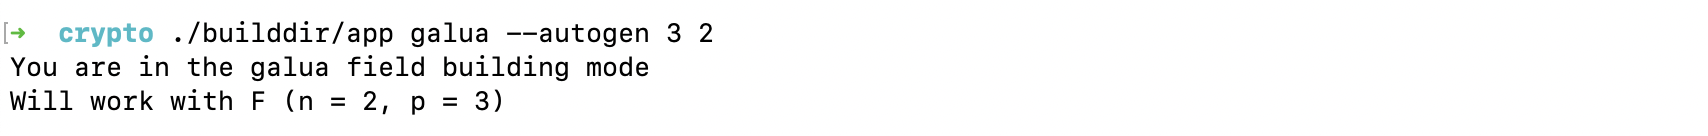
\includegraphics{14_1}
  \caption{Запуск}
\end{figure}

\begin{figure}[H]
  \centering
  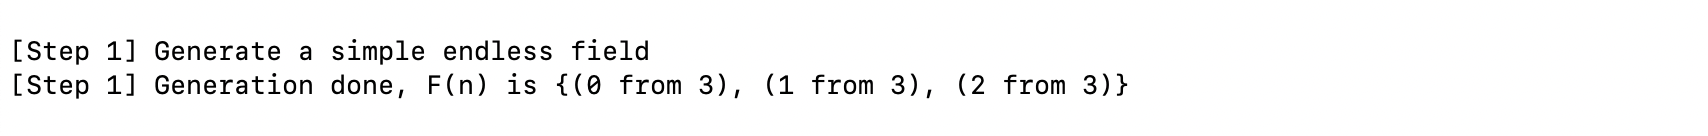
\includegraphics[width=1.4\textwidth]{14_2}
  \caption{Генерация $F_n = F_3$ над кольцом классов вычетов}
\end{figure}

\begin{figure}[H]
  \centering
  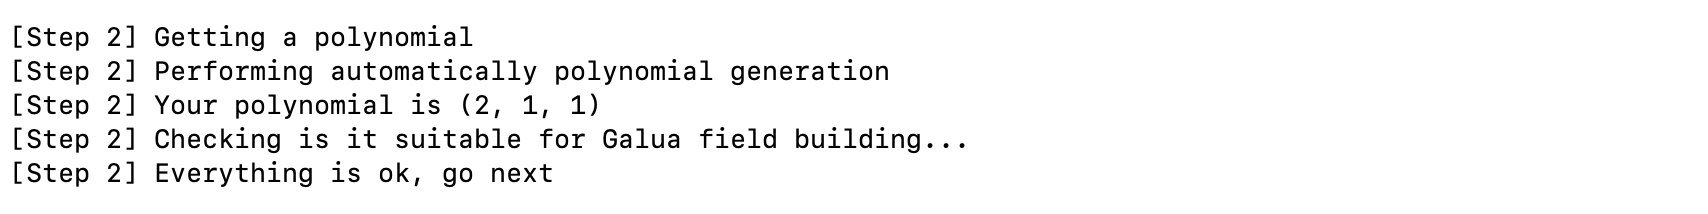
\includegraphics{14_3}
  \caption{Генерация неприводимого многочлена}
\end{figure}

\begin{figure}[H]
  \centering
  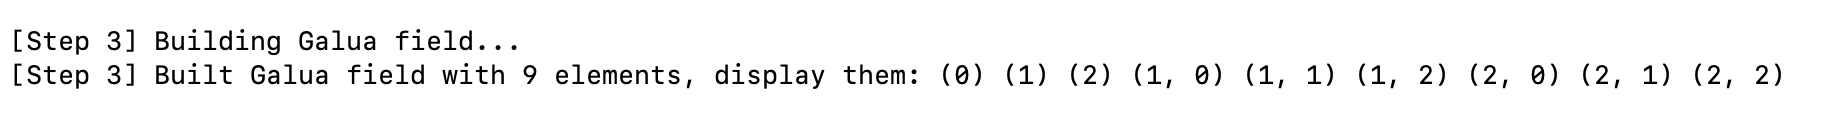
\includegraphics[width=\textwidth]{14_4}
  \caption{Элементы поля Галуа}
\end{figure}

\begin{figure}[H]
  \centering
  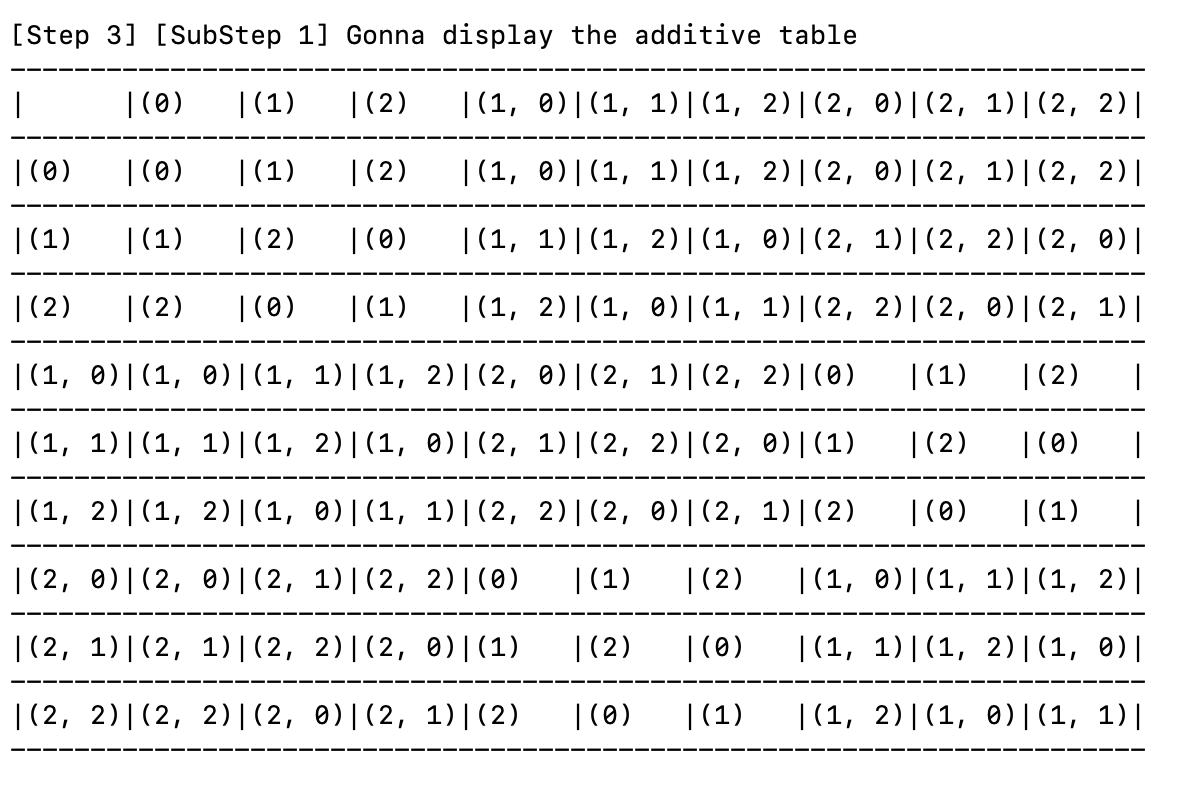
\includegraphics[width=\textwidth]{14_5}
  \caption{Сложение над элементами поля}
\end{figure}

\begin{figure}[H]
  \centering
  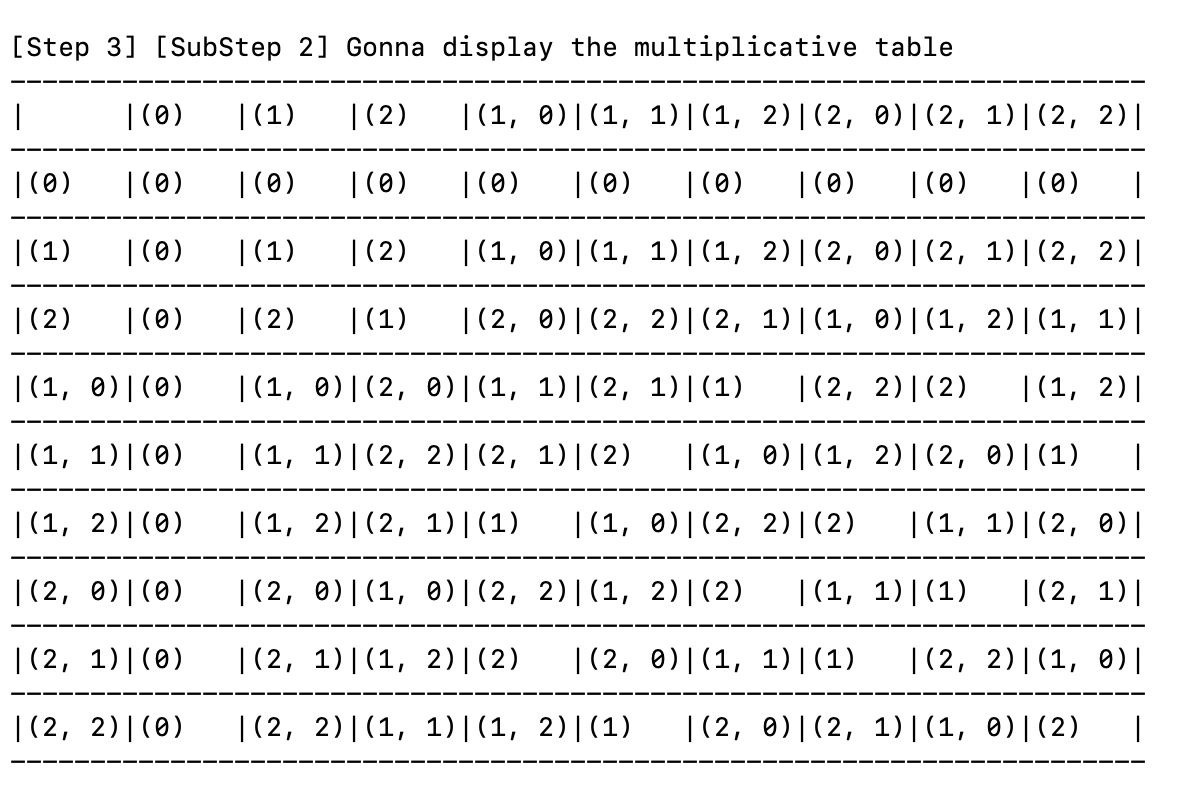
\includegraphics[width=\textwidth]{14_6}
  \caption{Умножение над элементами поля}
\end{figure}

\begin{figure}[H]
  \centering
  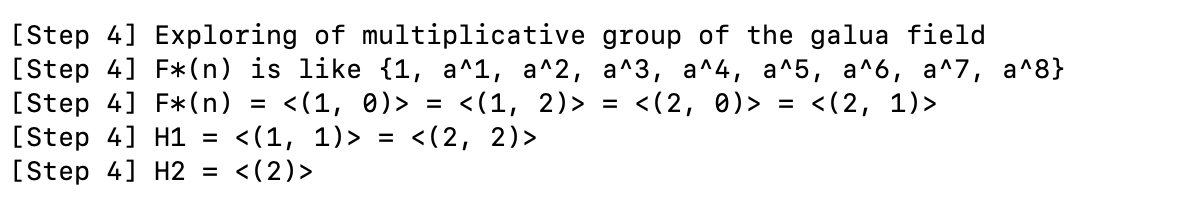
\includegraphics[width=\textwidth]{14_7}
  \caption{Исследование мултипликативной группы поля}
\end{figure}

\subsection{Афинный шифр}

\begin{figure}[H]
  \centering
  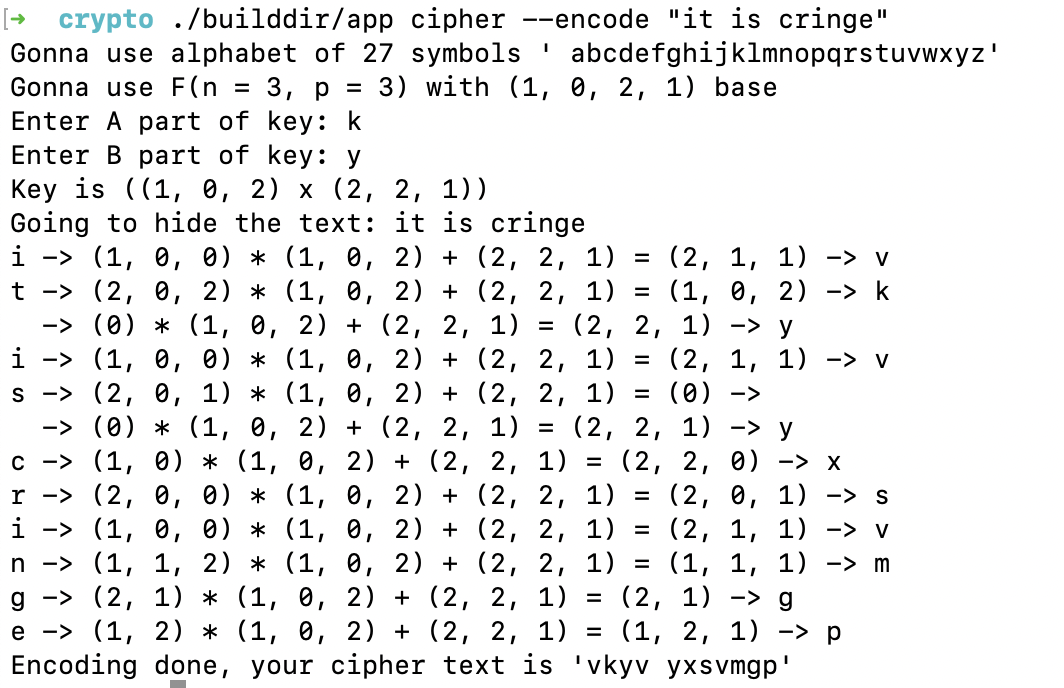
\includegraphics[width=\textwidth]{14_8}
  \caption{Зашифрование фразы "it is cringe" ключом (k, y)}
\end{figure}

\begin{figure}[H]
  \centering
  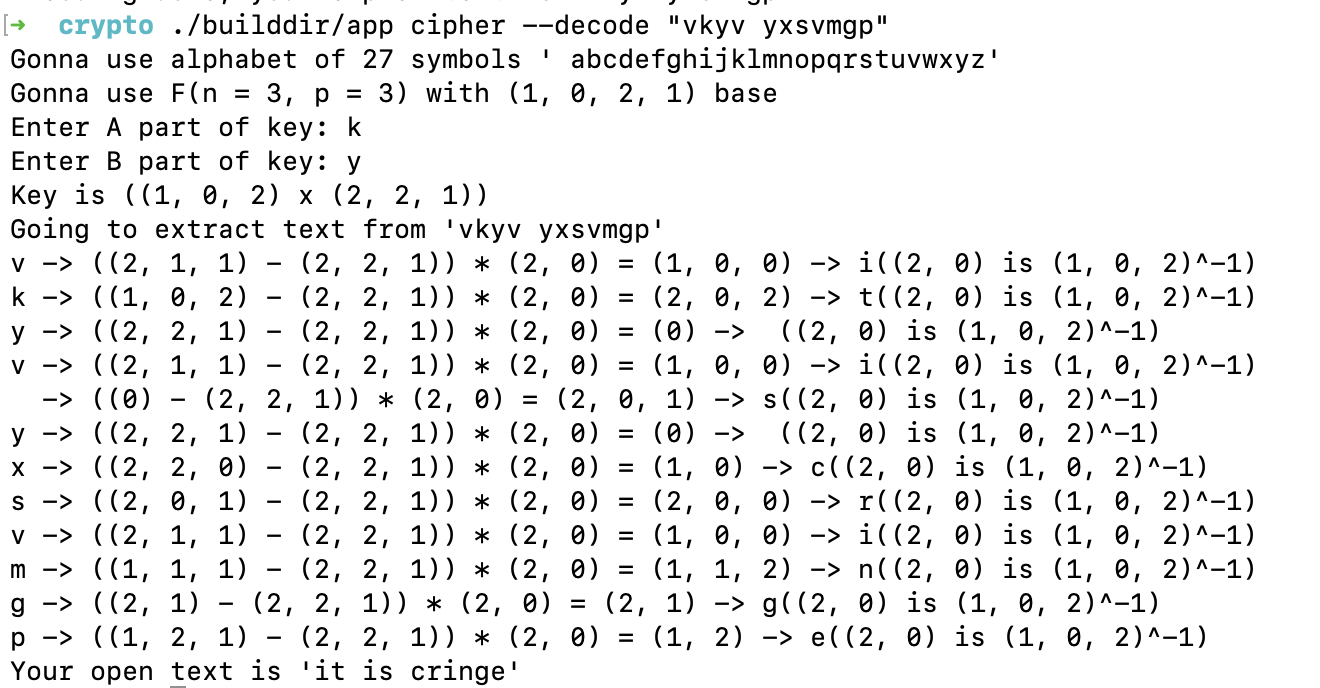
\includegraphics[width=\textwidth]{14_9}
  \caption{Успешное расшифрование тем же ключом}
\end{figure}

\newpage
\section{Выводы}

В ходе данной практической работы были реализованы средства для
рабо-ты с кольцами, многочленами и полями в т.ч. Галуа. Стало ясно,
что эти матема-тикие объекты можно успешно применять в криптографии, в том
числе для увеличения устойчивости к полному перебору, так как операции над
полем Галуа сложнее и вычислительно емче операций над целыми числами.

\end{document}
